\subsection{How little data is enough? (RQ3)}
\label{sec:res-scarcity}

\Cref{fig:scarmodel}\iffull{} and \cref{fig:scarsubset}\fi{} show RMSE on the fixed unseen test stations as the training set shrinks from about 474 stations (3,889 visits) to about 9 stations (75 visits). Each point averages 5 folds $\times$ 3 random station draws. Fold-averaged \R{} values for key settings are in \cref{tab:scarcity}\iffull, and full RMSE tables in \cref{app:tables}\fi.

\begin{figure}[t]
  \centering
  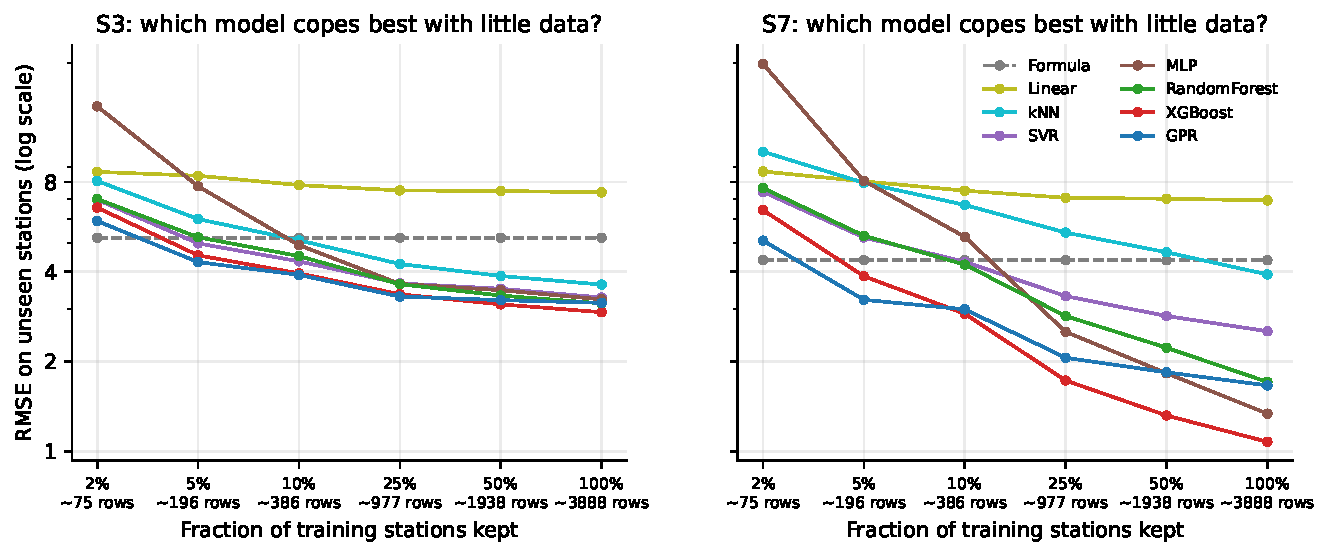
\includegraphics[width=\textwidth]{fig_scar_by_model.pdf}
  \caption{Data scarcity by model: RMSE on unseen stations (log scale) against the fraction of training stations kept, for \sub{S3} and \sub{S7}. Dashed grey: the renormalised formula, which needs no training data.}
  \label{fig:scarmodel}
\end{figure}

\iffull
\begin{figure}[t]
  \centering
  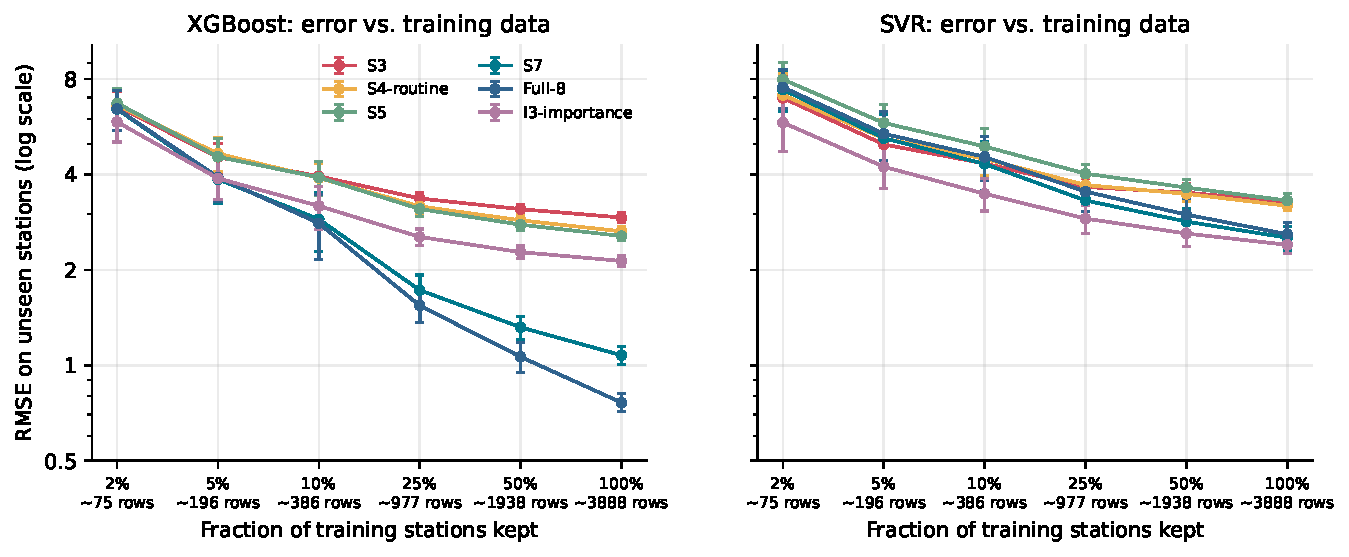
\includegraphics[width=\textwidth]{fig_scar_by_subset.pdf}
  \caption{Data scarcity by subset for XGBoost and SVR (error bars: s.d.\ over folds and repeats). With little data all subsets perform alike; the value of extra parameters is only realised with enough training stations.}
  \label{fig:scarsubset}
\end{figure}
\fi

\begin{table}[h]
\centering\small
\caption{Fold-averaged \R{} on unseen stations versus training-set size (mean number of training stations / visits).}
\label{tab:scarcity}
\begin{tabular}{llrrrrrr}
\toprule
& & 2\% & 5\% & 10\% & 25\% & 50\% & 100\% \\
Subset & Model & 9 / 75 & 24 / 196 & 47 / 387 & 118 / 977 & 237 / 1,939 & 474 / 3,889 \\
\midrule
\multirow{4}{*}{\sub{S3}} & Formula & \textbf{0.860} & 0.860 & 0.860 & 0.860 & 0.860 & 0.860 \\
 & GPR & 0.810 & \textbf{0.902} & \textbf{0.921} & \textbf{0.944} & 0.947 & 0.949 \\
 & XGBoost & 0.775 & 0.894 & 0.919 & 0.942 & \textbf{0.950} & \textbf{0.956} \\
 & MLP & $-0.619$ & 0.644 & 0.873 & 0.932 & 0.938 & 0.947 \\
\midrule
\multirow{3}{*}{\sub{I3}} & Formula & \textbf{0.873} & 0.873 & 0.873 & 0.873 & 0.873 & 0.873 \\
 & GPR & 0.860 & 0.918 & 0.941 & 0.960 & 0.967 & 0.969 \\
 & XGBoost & 0.821 & \textbf{0.922} & \textbf{0.947} & \textbf{0.967} & \textbf{0.973} & \textbf{0.977} \\
\midrule
\multirow{3}{*}{\sub{S7}} & Formula & \textbf{0.902} & 0.902 & 0.902 & 0.902 & 0.902 & 0.902 \\
 & GPR & 0.860 & \textbf{0.944} & 0.952 & 0.977 & 0.982 & 0.985 \\
 & XGBoost & 0.786 & 0.923 & \textbf{0.956} & \textbf{0.985} & \textbf{0.991} & \textbf{0.994} \\
\bottomrule
\end{tabular}
\end{table}

\paragraph{There is a minimum viable training set.} With only about 9 training stations (75 visits), \emph{no} learned model beats the renormalised formula for \sub{S3}: formula 0.860, best model (GPR) 0.810. The crossover lies between 9 and 24 stations. From about 24 stations (roughly 200 visits) onwards GPR and XGBoost beat the formula for every subset, and their advantage keeps growing. For \sub{S3} the curve flattens after about 118 stations (25\%). Doubling the training set beyond that buys only 0.01 in \R{}.

\paragraph{Which model to use depends on how much data there is.}
\begin{itemize}
  \item \textbf{Very scarce (fewer than about 50 stations):} GPR is the best or joint-best learner. Its smooth prior and explicit noise model regularise well, and it degrades most gracefully. At 2\% it retains category accuracy of 84.0\% on \sub{S3} and 91.1\% on \sub{Full-8}\optref{fig:scarheat}.
  \item \textbf{Moderate to rich data:} XGBoost takes over and keeps improving, especially for the larger subsets, where it has more interactions to learn.
  \item \textbf{Neural networks need data:} the MLP is the worst model at 2\% (\R{}\,$<0$, i.e.\ worse than predicting the mean) but competitive at 100\%. As anticipated in the methodology, this is an informative negative result for the data-scarce use case.
\end{itemize}

\paragraph{Extra parameters only pay off with enough data.} At 2--5\% all subsets give similar RMSE\optref{fig:scarsubset}. \sub{S7} and \sub{Full-8} separate from \sub{S3} only once about 50 or more training stations are available. The reason is that learning the five-dimensional shape of the extra sub-indices needs more examples. A sparsely monitored region therefore gains more from \emph{more stations} than from \emph{more parameters}, until about 50--100 stations.

\iffull
\begin{figure}[t]
  \centering
  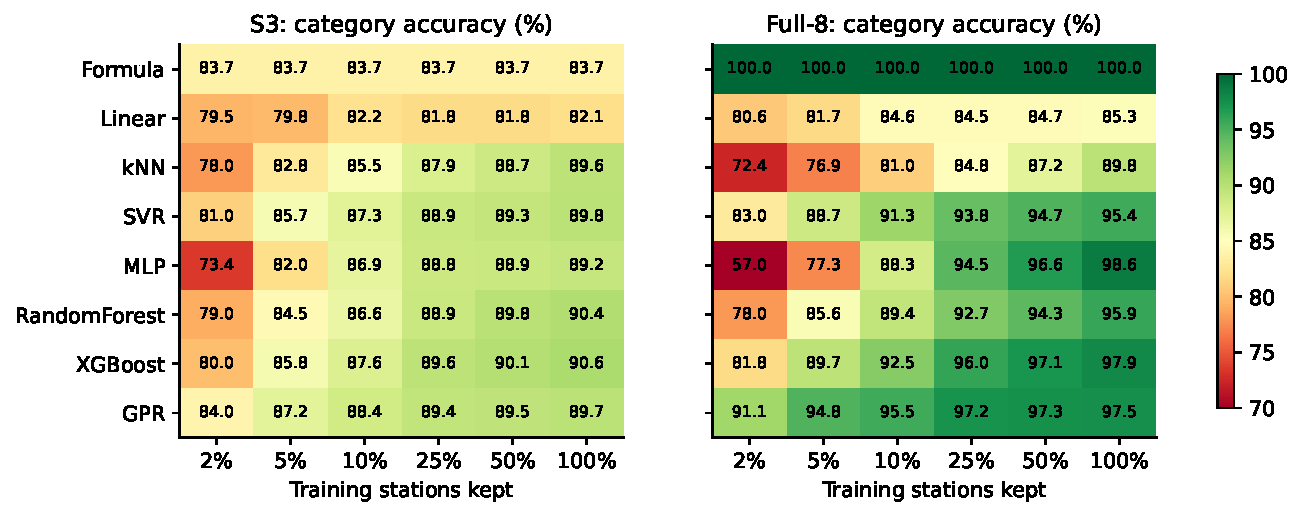
\includegraphics[width=\textwidth]{fig_scar_catacc_heatmap.pdf}
  \caption{Category accuracy (\%) on unseen stations by model and training size, for \sub{S3} (left) and \sub{Full-8} (right).}
  \label{fig:scarheat}
\end{figure}
\fi

\begin{keybox}[Finding 3]
A three-parameter model needs data from about \textbf{25 or more stations} (roughly 200 visits) to beat simply re-weighting the formula, and about \textbf{120 stations} to come within 0.01 \R{} of its full-data accuracy. Below that, use the formula or a GPR. With full training data, use XGBoost.
\end{keybox}
